\begin{figure}[!h]
  \vskip -0.25cm
  \begin{center}
    \ifshort
    %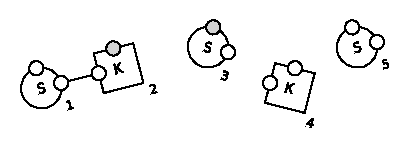
\includegraphics[scale=1.0]{figures/mixture-compact.pdf}
    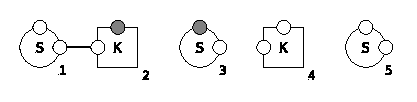
\includegraphics[scale=1.0]{figures/mixture-linear.pdf}
    \else
    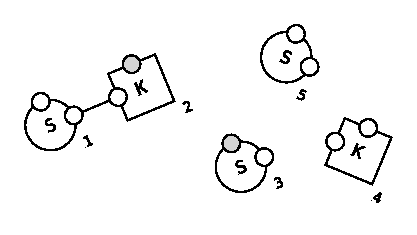
\includegraphics[scale=0.9]{figures/mixture.pdf}
    \fi
  \end{center}
  \vskip -0.5cm
  \caption{An example of a reaction mixture. Instead of naming sites,
    we here identify them by their position on
    agents\longversion{(phosphorylation sites are always shown on
      top). The relative position of agents in the figure is
    insignificant}.  Phosphorylated sites are shown in gray.  Number
    labels correspond to global agent identifiers. }
  \label{fig:mixture}
\end{figure}
